%File: q4.tex
%Date: Wed Jun 25 05:38:40 2014 +0800
%Author: Yuxin Wu <ppwwyyxxc@gmail.com>

\section{Query 4}
\begin{frame}{Query 4}
  Given $k$ , $t$ , where $t$ is used to define a subgraph $G′$ of $G$, find
  the top-$k$ centralized vertex in $G′$. Here the centrality for a
  vertex $v$ in a graph $G(V, E)$ is defined as:

  \[ C(v) = \dfrac{r(v)^2}{(|V| - 1) S(v)},\]
    where $ r(v)$ is \# of vertex reachable from $v$ (exclusive),
 $ S(v) = \sum_{u\in V} dist(u, v) $ is very expensive to calculate.

\end{frame}

\begin{frame}{Framework}
  General framework to obtain top-$k$ centrality:
  \begin{enumerate}
    \item
      Estimate an upper bound of $C(v)$
      for each $v$ and maintain them with a max-heap.

    \item

      Iteratively pop the top element from the heap and calculate
      its actual value. If the actual value is still the largest in
      heap, then it's certainly the largest among all actual values
      of remaining element. Otherwise we insert this actual value
      back to the heap.
      \begin{center}
        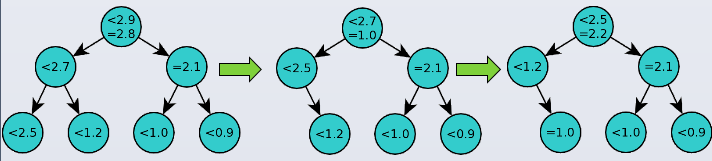
\includegraphics[width=0.9\textwidth]{res/heap.png}
      \end{center}
  \end{enumerate}

\end{frame}

\begin{frame}{Lower Bound of $ S(v)$}
  \[ S(v) \ge \sum_{dist(u, v) \le \ell}dist(u, v) + \sum_{dist(u,v)>\ell}(\ell + 1) \]

The first term is calculated by a BFS from $v$ with search depth
limited to $\ell$. The second term is obtained by counting.

To choose a proper $\ell$, we compare our current estimation of each
$S(v)$ to an approximation of $S(v)$ and increase $\ell$ when the mean-
square error is large. Since social networks have \textbf{small
  diameter(!)}, a small $\ell$ (3 or 4) is sufficient to guarantee a good
lower bound estimation of $S(v)$.

\end{frame}

\begin{frame}{Approximation of $ S(v)$}
Random sample a subset $ V_1$ of $ V$, and run a thorough BFS
on each of them, giving $ dist(u, v)$ for each $u \in V_1 $ and $ v \in V$. Then we
have:

\[ \forall v \in V, S(v) \approx \sum_{u\in V_1} dist(u, v)\dfrac{|V|}{|V_1|} \]

This is a highly accurate approximation, which gave an average
1$\sim$2\% error sampled with 0.1\% of $V$ in our experiments.

This approximation can also help with pruning: by calculating
actual centrality of the vertices with top-$(3k)$ approximated
centrality, we get $3k$ actual centrality that is very likely to
contain the actual top-$k$ centralities. Then the $k$th centrality
among the $3k$ results is a very good lower bound of the top-$k$ centrality.

\end{frame}
